%
% Copyright (c) 2020 Antonio Coín Castro
%
% This work is licensed under a
% Creative Commons Attribution-ShareAlike 4.0 International License.
%
% You should have received a copy of the license along with this
% work. If not, see <http://creativecommons.org/licenses/by-sa/4.0/>.

Having presented ordinary differential equations and their solutions in the previous chapter, we now focus on our main goal: the study and understanding of \textit{implicit} differential equations, that is, equations in which the derivative can't be isolated. Since we can't put this type of equations into explicit form, all the theory discussed earlier doesn't apply directly to this case, and thus we want to find a general framework that allows for the treatment of these equations from a theoretical point of view. For this task we will refer to \cite{petrovski1966ordinary} and \cite{arnold2012geometrical}.

Given that equations are expressed in the general or implicit form, it makes sense to think that the \textit{implicit function theorem} will play a significant role in disentangling the complexities behind this formulation of differential equations, and tell us something about their local behaviour. In an effort to provide all the necessary tools for the study we are about to undertake, we write down the statement of this famous theorem below.

\begin{theorem}[Implicit function theorem]
Let $G$ be an open set in $\R^{n+m}$ with coordinates $(x, y)$ and let $F:G \to \R^m$ be continuously differentiable. If $(a,b)\in G$ verifies $F(a,b)=0$ and the Jacobian matrix $\frac{\partial F}{\partial y}(a, b)$ is nonsingular, then there exists an open set $U \subset \R^n$ with $a \in U$ and a unique $\mathcal C^1$ function $f:U\to \R^m$ such that:
\begin{enumerate}
  \item $f(a)=b$;
  \item $F(x, f(x)) = 0$ for all $x$ in $U$;
  \item The Jacobian matrix of $f$ is given by the matrix product
  \[
    Jf(x) = - \left( \frac{\partial F}{\partial y}(x, f(x))\right)^{-1} \left( \frac{\partial F}{\partial x}(x, f(x)) \right), \quad x \in U.
  \]
\end{enumerate}
\end{theorem}

\begin{proof}
A standard proof employing the equally renowned inverse function theorem can be found in \cite[374]{apostol1974analysis}. The last differentiation formula is obtained by differentiating the expression $f(x, g(x)) = 0$ and applying the chain rule.
\end{proof}

Even though we have stated the theorem for arbitrary dimensions, we will only apply it when $n=2$ and $m=1$, making the Jacobian matrix a single partial derivative. In fact, we recover the notation established in the previous chapter, and henceforth consider a function $F:\R^3 \to \R$ and the associated differential equation
\begin{equation}\label{eq:ode-implicit}
  F(x,y,y') = 0.
\end{equation}
Also, following a standard notation, we will denote by $F_x$, $F_y$ and $F_p$ the partial derivatives of the function $F$ with respect to each of its three variables $x$, $y$ and $p$. Then, the theorem assumes the following form:

\begin{corollary} \label{cor:implicit}
  Let $G$ be an open subset of $\R^3$ and let $F:\R^3 \to \R$ be continuously differentiable. If $(x_0, y_0, p_0) \in G$ verifies $F(x_0, y_0, p_0) = 0$ and $F_p(x_0,y_0,z_0) \neq 0$, then there exists an open set $U\subset \R^2$ containing $(x_0, y_0)$ and a unique $\mathcal C^1$ function $f:U\to \R$ such that $z_0=f(x_0,y_0)$ and $F(x, y, f(x,y))=0$ for all $(x, y) \in U$. Moreover, the partial derivative of $f$ with respect to its second variable is given by
  \[
  \frac{\partial f}{\partial y}(x, y) = - \frac{F_y(x,y, f(x,y))}{F_p(x, y, f(x,y))}.
  \]
\end{corollary}

\section{Integral curves of implicit equations}

In this case we will start with an example. If we consider the differential equation
\begin{equation} \label{eq:ex1}
  (y')^2 = y,
\end{equation}
we should immediatly observe that this expression is an abbreviation for two distinct explicit differential equations: $y'=\sqrt y$ and $y'=-\sqrt y$, for $y\ge0$. Each of these equations produces a direction field, as seen in Figure \ref{fig:ex1}, and each of them separately satisfies an existence and uniqueness theorem on their domain, though clearly the uniqueness of solution fails when combining them. Nevertheless, we would like to examine this kind of equations as a whole, and establish general conditions for their treatment.

\begin{figure}[h!]
\centering
\begin{subfigure}{.6\textwidth}
  \centering
  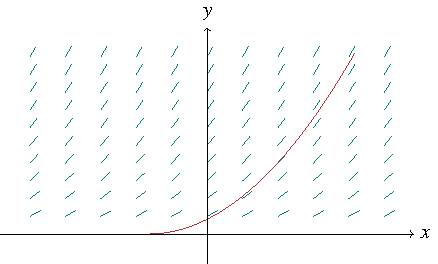
\includegraphics[width=\linewidth]{ex1}
\end{subfigure}
\begin{subfigure}{.6\textwidth}
  \centering
  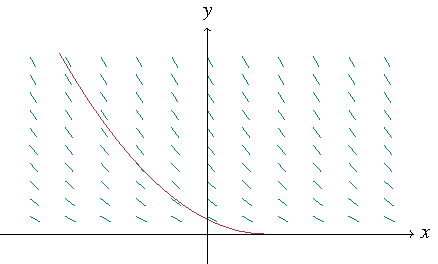
\includegraphics[width=\linewidth]{ex2}
\end{subfigure}
\caption{Direction fields of the two equations combined in the notation $(y')^2=y$.}
\label{fig:ex1}
\end{figure}

One thing to note from the beggining is that there are some occasions in which implicit equations can be put in explicit form, at least in theory. That is, there is a set of conditions that, when satisfied, guarantee that the equation is equivalent to another one in explicit form. Of course, in nontrivial cases this result will only hold locally, and as one would expect is a direct consequence of the aforementioned implicit function theorem.

\begin{theorem}
  Let $F:G \to \R$ be a continuously differentiable function on some domain $G$ of the $(x,y,p)$-space. Suppose that $(x_0,y_0,p_0) \in G$ simultaneously satisfies $F(x_0,y_0,p_0)=0$ and $F_p(x_0,y_0,p_0)\neq 0$. Then there exists a unique function $\phi$ defined on an interval containing $x_0$ that is a solution of the equation $F(x,y,y')=0$, satisfying $\phi(x_0)=y_0$ and $\phi'(x_0)=p_0$.
\end{theorem}

\begin{proof} Under these conditions we can apply Corollary \ref{cor:implicit} to $F(x,y,p)$ and express $p$ as a function of $x$ and $y$, that is, there exists a unique smooth $f$ such that $F(x,y,f(x,y))=0$ on a neighbourhood $U$ of the point $(x_0,y_0)$, that also verifies $p_0=f(x_0,y_0)$. Then the IVP
\[
  \begin{cases} y' = f(x,y) & \text{in } U,\\
    y(x_0)=y_0
  \end{cases}
\]
is well defined, and since $f_y$ is continuous, it verifies the conditions of Theorem \ref{th:picard}. Thus, there is a unique smooth function $\phi$ defined on a neighbourhood $I$ of $x_0$ such that $\phi'(x)=f(x, \phi(x))$ on $I$ and $\phi(x_0)=y_0$. This concludes the proof, seeing as how putting it all together we have
\[
p_0 = f(x_0, y_0) = f(x_0, \phi(x_0)) = \phi'(x_0)
\]
and
\[
F(x,\phi(x), \phi'(x)) = F(x, \phi(x), f(x, \phi(x))) = 0, \quad x \in I.
\]

\end{proof}

\begin{remark} Uniqueness of solution may fail if the requirement that $F_p\neq 0$ is not satisfied. For example, consider the equation
\[
(y')^2 - 2y' + 4y - 4x + 1 = 0,
\]
for which at the point $(0,0,1)$ we have $F_p=0$ but both $x$ and $x-x^2$ are valid solutions.
\end{remark}

If we take a closer look at the above result, we observe that for every choice of $p_0$ there is a potentially different solution to the equation. But just how many suitable points are there? Is there any condition that guarantees that the number of possible solutions passing through a given point in the plane is finite? The following theorem (cf. \cite[76]{petrovski1966ordinary}) gives a satisfactory answer, namely that we can limit the number of solutions in a neighbourhood if after setting a reference point $(x,y)$ we can solve the (algebraic) equation for $p$.

\begin{theorem} Given the differential equation
\begin{equation}\label{eq:implicit-th}
  F(x,y,y')=0,
\end{equation}
suppose that $F(x,y,p)$ is such that
\begin{enumerate}
  \item $F(x,y,p)$ is defined and continuously differentiable on a closed bounded domain $\bar{G}$ in $(x,y,p)$-space;
  \item At some point $(x_0,y_0)$ of the $(x,y)$-plane, equation \eqref{eq:implicit-th} has a finite number of distinct roots $p_1,\dots,p_m$ when solved for $p$;
  \item Each of the points $(x_0,y_0,p_i), i=1,\dots,m$ belongs to $G$ and has a neighbourhood in which $F(x,y,p)$ is continuously differentiable and satisfies $|F_p(x,y,p)|\ge c > 0$.
\end{enumerate}
Then there is a neighbourhood $\mathcal N$ of $(x_0,y_0)$ such that precisely $m$ solutions of \eqref{eq:implicit-th} pass through each point of $\mathcal N$.

\end{theorem}

\begin{proof}

\end{proof}

--------------->Cosas about $F$, $F_1$, etc.

As a final remark, we note that if we could algebraically solve for $y'$ (think for example that $F$ were a polynomial on $y'$) then we could not only establish the existence and uniqueness of solutions, but also determine exactly what these solutions were, as in the next example.

\begin{example} Let

\end{example}

\section{Geometrical approach to implicit equations}

When studying equations in implicit form, we can think of a geometrical approach that suggests considering the direction field not on the $(x,y)$-plane, but on the surface of the three-dimensional $(x,y,p)$-space given by the equation $F(x,y,p)=0$, where $p=dy/dx$. This way, even though the equation might define several direction fields, we compensate for this by adding a new dimension in which to visualize them together. This space is known as the space of \textit{1-jets} of functions $y(x)$, which is basically representing the truncated Taylor polynomial of a (differentiable) function at a given point.
